 \section{Sensores}
	Los sensores son dispositivos que permiten a los robots percibir su entorno y obtener información sobre su posición, movimiento, temperatura, proximidad, presión, entre otros aspectos. Estos sensores convierten datos físicos en señales eléctricas que el robot puede procesar para tomar decisiones o realizar tareas.

Se clasifican en:

	\subsection{Sensores Internos}
		\begin{enumerate}
			\item \textbf{Posición}
			
			Los sensores de posición miden la posición de cada articulación, es decir, el ángulo de articulación de un robot. A partir de dichos ángulos puede encontrarse la configuración del ejecutor final, y ubicar su posición y orientación por medio de la cinemática directa.\cite{saha2010robotics}\\
			
			
			\begin{enumerate}
				\item Lineal y rotativo
				\begin{enumerate}
					\item \textbf {Éncoders}: Es un dispositivo óptico digital que convierte el movimiento en una secuencia de pulsos digitales. Mediante el conteo de un solo bit o la decodificación de un conjunto de bits, los pulsos pueden convertirse en medidas relativas o absolutas. De este modo, los encóders son de tipo incremental o absoluto. Además, cada tipo puede ser lineal y rotatorio a su vez.\cite{saha2010robotics}\\
			
			\begin{enumerate}
				\item \underline{Éncoder lineal incremental:} Tiene una
				escala transparente con una retícula opaca. El tamaño del espesor de las líneas de la retícula y el del espacio entre ellas son iguales. De un lado, la escala se equipa con una fuente de luz y un lente de condensador. Del otro, hay celdas sensibles a la luz. La resistencia de las celdas (fotodiodos) disminuye cada vez que reciben un rayo de luz. De este modo, se genera un pulso cada vez que un rayo de luz es atravesado por la línea opaca. Este pulso se introduce en el controlador que actualiza a un contador \cite{saha2010robotics}.
				\\
				\\
				\\
				\\
				\\
				\\
				\\
		\begin{figure}[h]
	\centering
		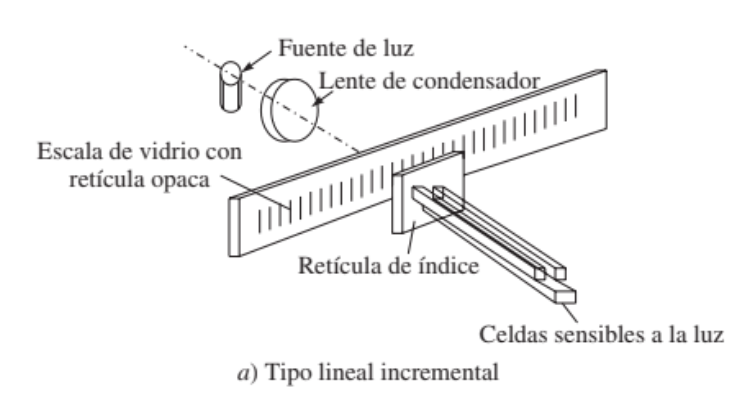
\includegraphics[width=0.6\textwidth]{Encoder_lineal_incremental.png}%
		\label{fig:Encoder_lineal_incremental}
		\cite{saha2010robotics}
	\caption{Imagen de encoder lineal incremental}
	\hfill
\end{figure}				

				\item \underline{Éncoder lineal absoluto}: En principio, se parece al encóder lineal incremental.  La diferencia es que da un valor absoluto de la distancia recorrida en cualquier momento. Así,
				las posibilidades de perder los pulsos a altas velocidades son menores. La salida es digital
				en este caso. La escala se marca con una secuencia de tiras opacas y transparentes. Si el bloque opaco que aparece en la escala de la ilustración (b)  representa 1 (uno) y el bloque transparente 0 (cero), entonces la columna de la extrema izquierda mostrará un número binario como 00000, es decir, un valor decimal de 0, y la columna siguiente mostrará un número binario 00001, es decir, una valor decimal de 1.\cite{saha2010robotics}
				
				\begin{figure}[h]
					\centering
					\subfloat[Función Encoder Lineal Absoluto]{%
						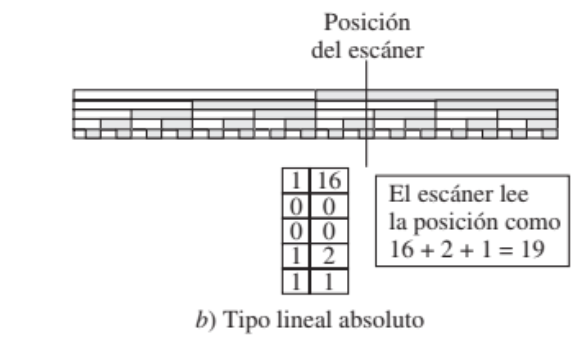
\includegraphics[width=0.4\textwidth]{Encoder_lineal_absoluto.png}%
						\label{fig:Función Encoder Lineal Absoluto}
						\cite{saha2010robotics}
					}
					\hfill
					\subfloat[Encoder lineal]{%
						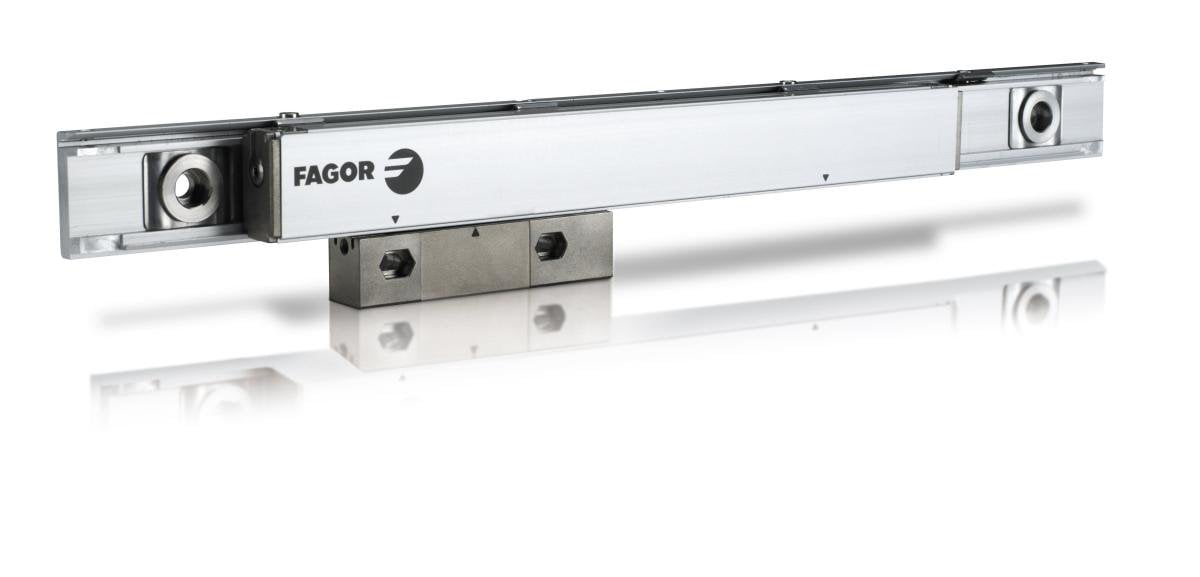
\includegraphics[width=0.4\textwidth]{Encoder_lineal_absoluto_2.png}%
						\label{fig:Encoder Lineal}
						
					}
					\caption{Imagen del funcionamiento del Éncoder lineal absoluto (a) e imagen de un éncoder lineal (b)}
					\label{fig:Encoders lineales}
				\end{figure}
				
				\item \underline{Éncoder rotativo incremental}: Se parece al encóder incremental lineal, con la diferencia
				de que las retículas se encuentran en este caso en un disco. El valor común del espesor de los espacios transparentes es igual a 20 micrones. Hay dos conjuntos de líneas de retículas en diferentes círculos que detectan el sentido de rotación, lo que permite mejorar la precisión del sensor. Hay otro círculo que sólo contiene una marca de retícula. Éste se usa para la medición del número
				de revoluciones completadas.\cite{saha2010robotics}
				\\
				\begin{figure}[h]
	\centering
	\subfloat[ Éncoder rotativo incremental]{%
		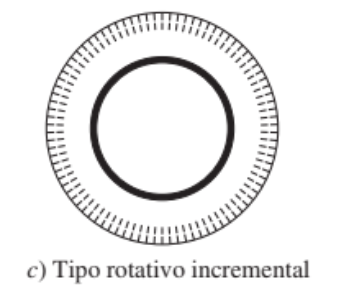
\includegraphics[width=0.4\textwidth]{Encoder_rotativo_incremental.png}%
		\label{fig:Encoder rotativo incremental}
		\cite{saha2010robotics}
	}
	\hfill
	\subfloat[Éncoder rotativo función]{%
		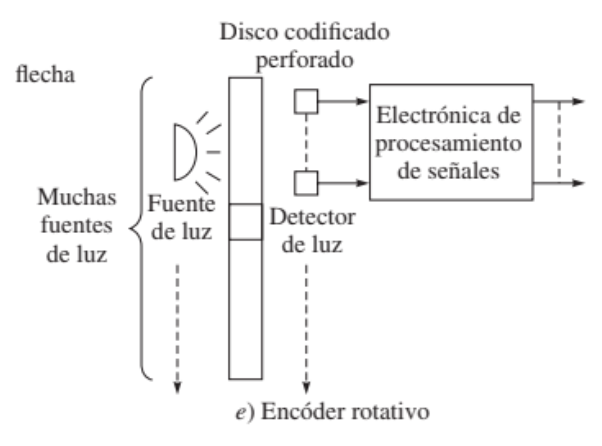
\includegraphics[width=0.4\textwidth]{Encoder_rotativo.png}%
		\label{fig:Encoder rotativo}
		\cite{saha2010robotics}
	}
	\caption{Imagen de la función del encoder rotativo incremental (a) y su principio (b)}
	\label{fig:Encoders}
\end{figure}				
\\
				\item \underline{Éncoder rotativo absoluto}: El disco se divide en un número de tiras circulares, y cada tira tiene segmentos de arco definidos, como se muestra en la figura. Este sensor proporciona directamente la salida digital (absoluta). El encóder se monta directamente sobre el eje del motor o con algún engranaje para aumentar la precisión de medición. Con el fin de evitar ruidos en este encóder, a veces se usa una escala gris. Un código gris, a diferencia de los códigos binarios, permite que sólo uno de los bits binarios en una secuencia de código cambie entre líneas radiales. También impide que se confundan los cambios en la salida binaria del encóder absoluto cuando el encóder oscila entre puntos. \cite {saha2010robotics}
				\\
				\begin{figure}[h]
					\centering
					\subfloat[Función éncoder rotativo absoluto]{%
						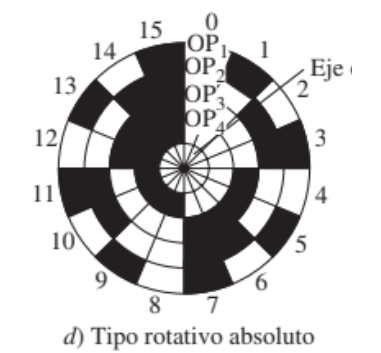
\includegraphics[width=0.4\textwidth]{Encoder_rotativo_absoluto.png}%
						\label{fig:Encoder absoluto}
						\cite{saha2010robotics}
					}
					\hfill
					\subfloat[Éncoder rotativo físico]{%
						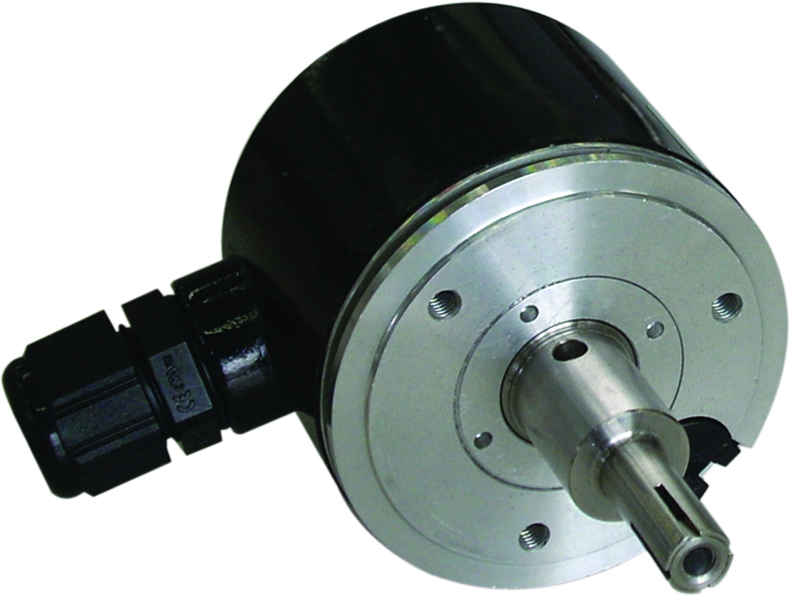
\includegraphics[width=0.4\textwidth]{Encoder_rotativo_2.png}%
						\label{fig:Encoder rotativo}
					}
					\caption{Imagen de la función del encoder rotativo absoluto (a) y su foto física (b)}
					\label{fig:mascotas}
				\end{figure}
				\\
				\\
				\\
			\end{enumerate}
			     
		     
					\item \textbf{Potenciómetro}: Es un dispositivo de resistencia variable que expresa desplazamientos lineales o angulares en términos de voltaje, tal como se muestra en las figuras a) y b), respectivamente. Consiste en una clavija deslizante que hace contacto con un elemento resistivo; conforme se mueve este punto de contacto, la resistencia entre el contacto deslizante y las conexiones de los extremos del dispositivo cambia en proporción al desplazamiento, x y  para potenciómetros lineales
					y angulares, respectivamente. \cite{saha2010robotics}
					
				\begin{figure}[h]
					\centering
					\subfloat[Potenciómetro lineal]{%
						\includegraphics[width=0.4\textwidth]{potenciometro_lineal.png}%
						\label{fig:potenciometro lineal}
						\cite{saha2010robotics}
					}
					\hfill
					\subfloat[Potenciómetro rotativo]{%
						\includegraphics[width=0.4\textwidth]{potenciometro_rotativo.png}%
						\label{fig:potenciometro rotativo}
						\cite{saha2010robotics}
					}
					\caption{Imagen del funcionamiento del potenciometro lineal (a) y rotativo (b).}
					\label{fig:Potenciometro}
				\end{figure}

\vspace{10mm}
			\item \textbf{LVDT}: Es uno de los transductores de desplazamiento más utilizados, especialmente cuando se requiere alta precisión. Este dispositivo genera una señal de corriente alterna (CA) cuya magnitud está directamente relacionada con el desplazamiento de un núcleo móvil.
		
		El principio de funcionamiento del LVDT se basa en un núcleo férrico que se mueve dentro de un campo magnético, el cual se genera de manera similar al de un transformador convencional. El sistema consta de una bobina primaria y dos bobinas secundarias idénticas dispuestas alrededor del núcleo. A medida que el núcleo cambia de posición con respecto a las bobinas, la distribución del campo magnético varía, lo que modifica la amplitud del voltaje inducido en las bobinas secundarias en función del desplazamiento del núcleo a lo largo de un determinado rango.\cite{saha2010robotics}
		\\
		
		\textbf{Ventajas:}
		\begin{itemize}
			\item Alta linealidad y sensibilidad.
			\item Respuesta dinámica elevada.
			\item Bajo rozamiento y desgaste mecánico.
			\item Usado en mediciones de pequeños desplazamientos con alta precisión.
			\item Se emplea en instrumentos de laboratorio, pruebas estructurales y monitoreo de vibraciones.
			\\
			\\
			\\
			\\
			\\
			\\
			\\
			\\
		\end{itemize}
		
		\begin{figure}[!h]
			\centering
			\subfloat[Operación de un LVDT]{%
				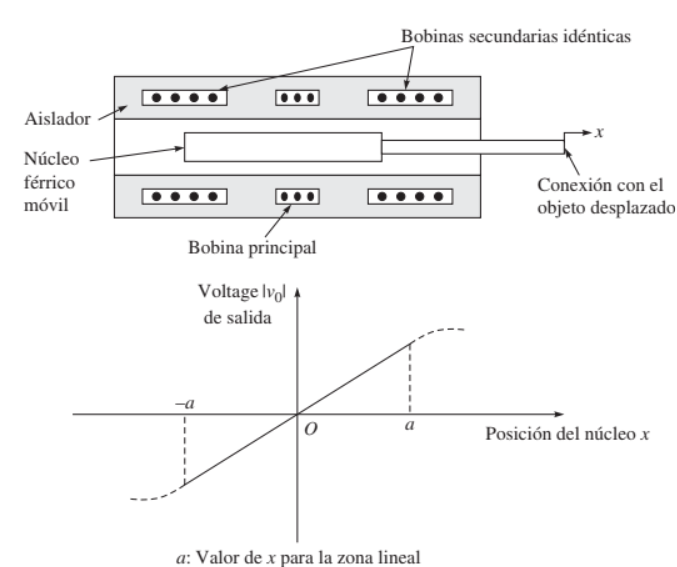
\includegraphics[width=0.6\textwidth]{LVDT.png}%
				\label{fig:LVDT}
				\cite{saha2010robotics}
			}
			\caption{Imagen de LVDT}
			\label{fig:figura_sensores}
		\end{figure}
\medspace		

			
			\item \textbf{Resólver y Sincronizador}: Mientras que los encoders generan señales digitales, los sincronizadores y resólvers proporcionan señales analógicas como salida. Estos dispositivos están compuestos por un eje giratorio (rotor) y una carcasa estacionaria (estator). Para su procesamiento en una computadora, sus señales deben convertirse a formato digital mediante un convertidor analógico-digital (ADC).
			
			 Los sincronizadores y resólvers utilizan rotores con un solo devanado que giran dentro de estatores fijos. En un sincronizador sencillo, el estator posee tres devanados dispuestos a 120° entre sí y conectados en configuración “Y”. Los resólvers, en cambio, tienen solo dos devanados en el estator, orientados a 90°. Debido a esta diferencia, \textit {los sincronizadores son más complejos y costosos de fabricar en comparación con los resólvers.}
			
			Los resólvers modernos pueden prescindir de escobillas, ya que emplean un transformador para acoplar las señales del rotor al estator. En este diseño, el devanado primario del transformador se encuentra en el estator y el secundario en el rotor. Sin embargo, algunos resólvers aún utilizan escobillas o anillos colectores tradicionales para transmitir la señal. Los resólvers sin escobillas son más resistentes, ya que eliminan el riesgo de desgaste mecánico, lo que prolonga su vida útil, limitándola únicamente por el desgaste de los cojinetes.\cite{saha2010robotics} \\
			\\
			\\
			\\
			\\

\begin{figure}[!h]
	\centering
	\subfloat[Resólver y Sincronizador]{%
		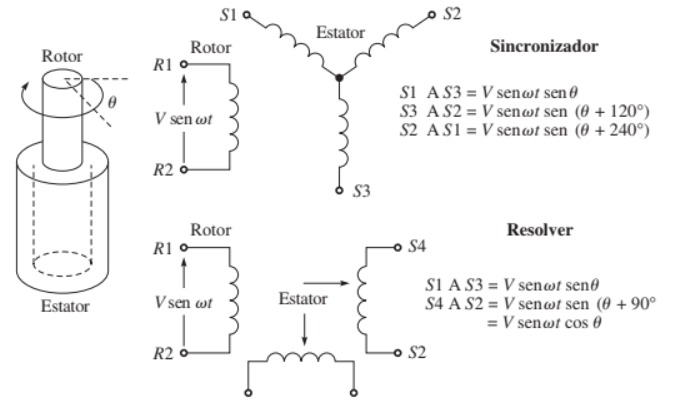
\includegraphics[width=0.6\textwidth]{Resolver_sincro.png}%
		\label{fig:sensores}
		\cite{saha2010robotics}
	}
	\caption{Imagen de Résolver y Sincronizador}
	\label{fig:Resolver_sinc}
	
	
\end{figure}
		
				\end{enumerate}
			\end{enumerate}
\vspace{10mm}
			\item \textbf{Velocidad}: Los sensores de velocidad realizan la medición tomando medidas de posición consecutivas a intervalos de tiempo constante, calculando la razón de cambio respecto al tiempo de los valores de posición, o lo determina en forma directa con base en diferentes principios.\cite{saha2010robotics}\\
           
			
			\begin{enumerate}
				\item Todos los sensores de posición:
				Básicamente todos los sensores de posición, cuando se utilizan con ciertos límites de tiempo, pueden dar la velocidad, por ejemplo, el número de pulsos proporcionados por un encóder de posición incremental dividido entre el tiempo consumido en hacerlo. Sin embargo, este método impone una carga computacional sobre el controlador, que podrá estar ocupado por algunas otras operaciones.\\
		
		\begin{figure}[!ht]
			\centering
			\subfloat[Sensores de posición]{%
				\includegraphics[width=0.4\textwidth]{Velocidadsensoresdeposición.jpg}%
				\label{fig:sensores}
				\cite{Sensordeposición}
				
				
			}
			\hfill
		\end{figure}
				
				\item Tacómetro: Estos sensores pueden encontrar directamente la velocidad en cualquier momento y sin mucha carga computacional. Éstos miden la velocidad de rotación de un elemento. Hay varios tipos de tacómetros en uso, pero un diseño sencillo se basa en la regla de Fleming, que declara que “el voltaje producido es proporcional al índice del acoplamiento inductivo”. Aquí un conductor (básicamente una bobina) se sujeta al elemento rotativo que gira en un campo magnético (estator). Conforme incrementa la velocidad del eje, el voltaje producido en las terminales de las bobinas también aumenta.\cite{saha2010robotics}\\
				
				\begin{figure}[h]
					\centering
					\subfloat[Tacómetro]{%
						\includegraphics[width=0.3\textwidth]{Tacómetro.jpg}%
						\label{fig:Tacómetro}
						\cite{Tacómetro}
					}
					\hfill
				\end{figure}
				
				\item Sensor de efecto Hall: Es un dispositivo que se utiliza para medir la magnitud de un campo magnético. Su función se basa en el fenómeno físico conocido como el efecto Hall, por el cual se genera una diferencia de potencial eléctrico, o voltaje Hall, a través de un material conductor cuando este se encuentra dentro de un campo magnético y se le hace pasar una corriente eléctrica. Este fenómeno fue descubierto en 1879 por el físico estadounidense Edwin Hall.\cite{Hall} \\
				
			\begin{figure}[h]
				\centering
				\subfloat[EfectoHall]{%
					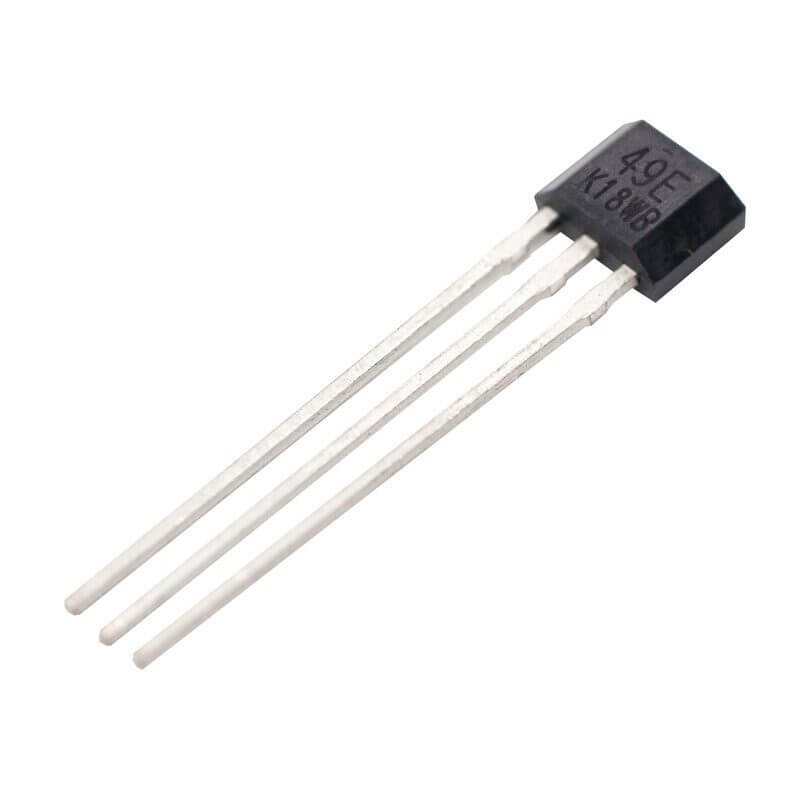
\includegraphics[width=0.25\textwidth]{Hall.jpg}%
					\label{fig:Hall}
					\cite{EfectoHall}
				}
				\hfill
			\end{figure}
			
			\end{enumerate}
			
			\item \textbf{Aceleración}
			
			Los Sensores de aceleración son dispositivos que mide la aceleración experimentada por un objeto en movimiento. Funciona detectando cambios en la velocidad del objeto en una dirección particular. Cuando un objeto acelera, cambia su velocidad en esa dirección, y el sensor de aceleración registra este cambio. \cite{Aceleración} \\
			
			\begin{enumerate}
				\item Todos los sensores de fuerza: De manera parecida a las mediciones de velocidad que se dan a partir de la información de los sensores de posición, pueden encontrarse las aceleraciones como la razón de cambio respecto al tiempo de las velocidades obtenidas por los sensores de velocidad o calculado a partir de las informaciones de posición. Pero ésta no es una manera efi ciente para calcular la aceleración, puesto que impondrá una carga de trabajo pesada sobre la computadora, lo que puede reducir la velocidad de operación del sistema. Otra forma de medir la aceleración es calculando la fuerza que resulta de multiplicar masa por aceleración. \cite{saha2010robotics}\\
			\end{enumerate}
				\begin{figure}[h]
				\centering
				\subfloat[Aceleración]{%
					\includegraphics[width=0.25\textwidth]{Aceleración.jpg}%
					\label{fig:Aceleración}
					\cite{Aceleración}
				}
				\hfill
			\end{figure}
			
			\item \textbf{Fuerza}
			
			Una balanza de resorte es un ejemplo de un sensor de
			fuerza en donde se aplica una fuerza, por ejemplo, el peso, al platillo de balanza que causa un desplazamiento, es decir, el resorte se estira. El desplazamiento es entonces una medida de la fuerza. Existen otros tipos de sensores de fuerza, por ejemplo, con base en galgas, utilizando el sensor de efecto Hall, etcétera. \cite{saha2010robotics}\\
			\begin{enumerate}
				\item Galgas extensométricas: Es un componente eléctrico que convierte la deformación en un cambio de resistencia eléctrica. La deformación se puede medir mediante tracción, compresión, torsión, cortante o flexión. La resistencia eléctrica de la mayoría de las galgas extensométricas cambia debido a la tensión mecánica, la tensión térmica o la tensión residual. Aplicando una galga extensiométrica a un material podemos medir su tensión, los cambios de forma o cuándo se produce la deformación. \cite{Galgas}\\
				
				\begin{figure}[h]
					\centering
					\subfloat[Galgas]{%
						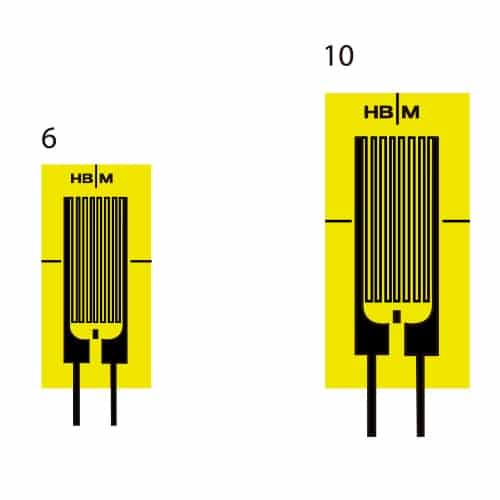
\includegraphics[width=0.25\textwidth]{Galgas.jpg}%
						\label{fig:Galgas}
						\cite{GalgasImagen}
					}
					\\
					\hfill
					\\

				\end{figure}
				
				\item Interruptores de efecto Hall: Un interruptor de efecto Hall funciona midiendo la intensidad de un campo magnético cercano. Cuando un campo magnético se aplica cerca del material sensibilizado por el efecto Hall, éste produce una diferencia de potencial en los bordes opuestos, que se puede medir y utilizar para activar o desactivar el interruptor. La sensibilidad y la precisión del interruptor dependen del material utilizado y de las condiciones del campo magnético.\cite{Efecto_Hall}\\
				\\
				\\
				\\
				\\
				
				\begin{figure}[h]
					\centering
					\subfloat[EfectoHall]{%
						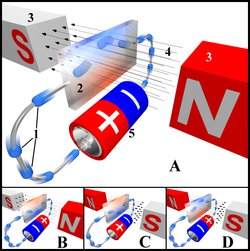
\includegraphics[width=0.25\textwidth]{EfectoHall.jpg}%
						\label{fig:EfectoHall}
						\cite{Efecto_Hall}
					}
					\hfill
				\end{figure}
				
				\item Interruptores piezoeléctricos: Un material piezoeléctrico presenta un fenómeno conocido como efecto piezoeléctrico. Este efecto señala que cuando cristales elásticos asimétricos se deforman mediante una fuerza, se desarrollará un potencial eléctrico dentro de la red cristalina deformada. \cite{saha2010robotics}\\
				
					\begin{figure}[h]
					\centering
					\subfloat[Piezoelectrico]{%
						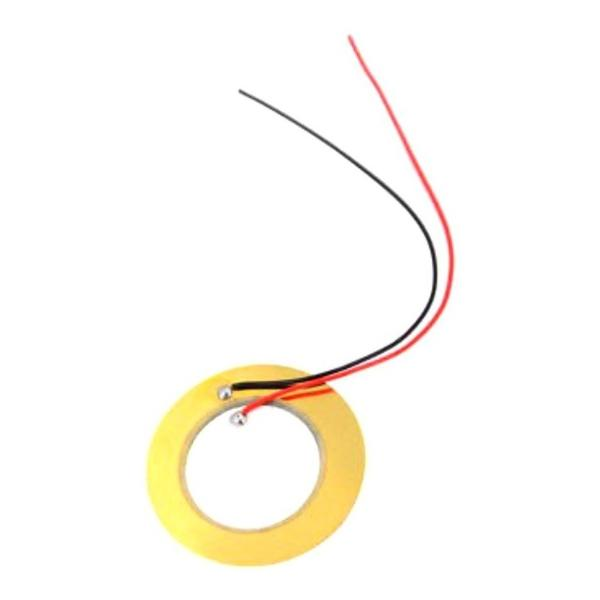
\includegraphics[width=0.25\textwidth]{Piezoelectrico.jpg}%
						\label{fig:Piezoelectrico}
						\cite{Piezoelectrico}
					}
					\hfill
				\end{figure}
				
			\end{enumerate}
		\end{enumerate}
		
	\subsection{Sensores Externos}
	 \begin{enumerate}
		\item \textbf{Tipo de contacto}
		\begin{enumerate}
			\item Interruptores de límite
			\item Interruptores neumáticos
			\item Sensores piezoeléctricos
			\item Transductores de presión
		\end{enumerate}
		\item \textbf{Tipo sin contacto}
		\begin{enumerate}
			\item Sensores de proximidad:  Es un dispositivo que detecta la presencia o ausencia de un objeto dentro de un rango específico sin necesidad de contacto físico. Este tipo de sensor es ampliamente utilizado en aplicaciones industriales y de automatización debido a su capacidad para operar en entornos donde el contacto directo podría ser problemático o dañino.\cite{Prox}\\ 
			\begin{figure}[h]
				\centering
				\subfloat[Sensor de proximidad]{%
					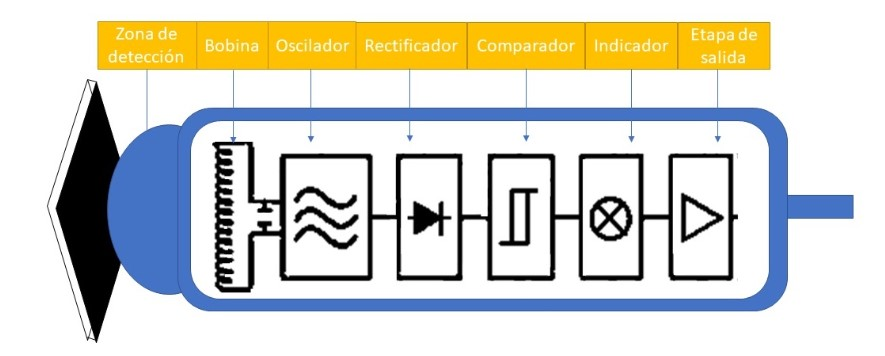
\includegraphics[width=0.20\textwidth]{Prox.jpg}%
					\label{fig:Sensor de proximidad}
					\cite{Prox}
				}
				\hfill
			\end{figure}
			\item Sensores de efecto Hall: Es un dispositivo que utiliza el efecto Hall para detectar campos magnéticos y convertir esta medición en una señal eléctrica. Este tipo de sensor es particularmente útil en aplicaciones donde se requiere la detección de la proximidad o la posición de objetos magnéticos sin necesidad de contacto físico.\cite{EHall}\\ 
			\begin{figure}[h]
				\centering
				\subfloat[Sensor de efecto Hall]{%
					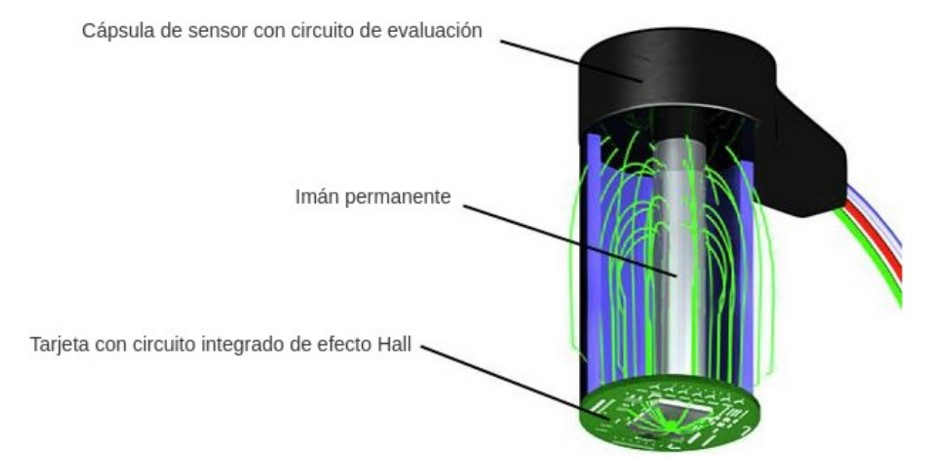
\includegraphics[width=0.20\textwidth]{SHall.jpg}%
					\label{fig:Sensor de efecto Hall}
					\cite{EHall}
				}
				\hfill
			\end{figure}
			\item Sensores de microondas: son dispositivos electrónicos que utilizan radiación de microondas para detectar movimiento, presencia o distancia sin necesidad de contacto físico. Estos sensores son especialmente útiles en aplicaciones donde la detección sin contacto es crucial, como en sistemas de seguridad, automatización industrial y control de tráfico.\cite{microo}\\ 
			\begin{figure}[h]
				\centering
				\subfloat[Sensores de microondas]{%
					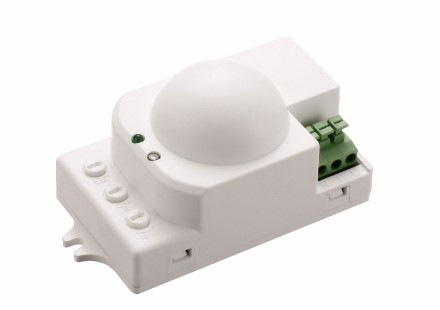
\includegraphics[width=0.20\textwidth]{Microoondas.jpg}%
					\label{fig:Sensores de microondas}
					\cite{microo}
				}
				\hfill
			\end{figure}
			\item Sensores ultrasónicos: Son dispositivos que utilizan ondas sonoras de alta frecuencia para medir distancias y detectar objetos sin contacto físico. Estos sensores son particularmente útiles en aplicaciones industriales y automatización, donde la precisión y la fiabilidad son esenciales.\cite{ultrason}\\ 
			\begin{figure}[h]
				\centering
				\subfloat[Sensores ultrasónicos]{%
					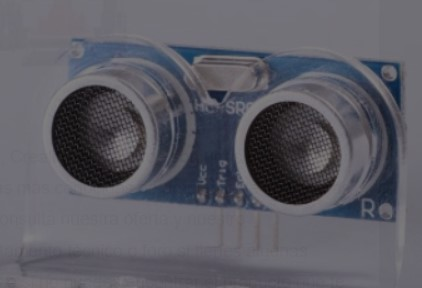
\includegraphics[width=0.20\textwidth]{Ultrasonico.jpg}%
					\label{fig:Sensores ultrasónicos}
					\cite{ultrason}
				}
				\hfill
			\end{figure}
			\item Sensores láser: Son dispositivos ópticos que utilizan un haz de luz láser para medir distancias, posiciones y detectar objetos sin contacto físico. Su capacidad para operar sin necesidad de tocar el objeto a medir los convierte en herramientas valiosas en diversas aplicaciones industriales y tecnológicas.\cite{Slaser}\\ 
			\begin{figure}[h]
				\centering
				\subfloat[Sensores láser]{%
					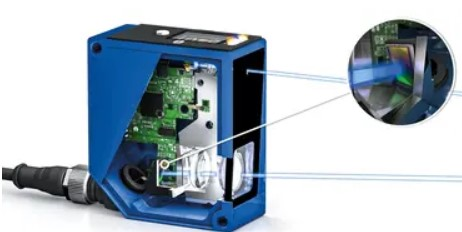
\includegraphics[width=0.15\textwidth]{SensorLaser.jpg}%
					\label{fig:Sensores láser}
					\cite{Slaser}
				}
				\hfill
			\end{figure}
			\item Sensores de visión: Son dispositivos que utilizan tecnología de imagen para detectar y analizar objetos sin necesidad de contacto físico. Estos sensores son parte integral de los sistemas de visión artificial y se emplean en diversas aplicaciones industriales, como inspección de calidad, control de procesos y automatización.\cite{Svision}\\ 
			\begin{figure}[h]
				\centering
				\subfloat[Sensores de visión]{%
					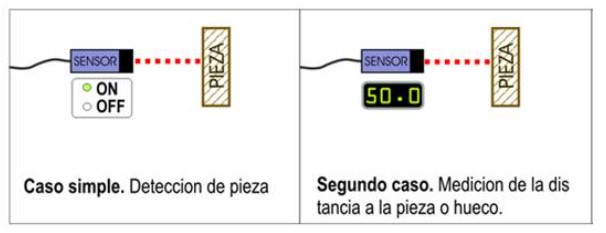
\includegraphics[width=0.20\textwidth]{SensorVision.jpg}%
					\label{fig:Sensores de visión}
					\cite{Svision}
				}
				\hfill
			\end{figure}
		\end{enumerate}
	\end{enumerate}

Para usar dos imágenes como en \autoref{fig:mascotas}, se utilizó \texttt{subfloat}.
% Dos imágenes de mascotas
\begin{figure}[h]
	\centering
	\subfloat[Perro]{%
		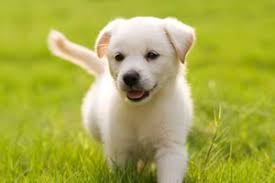
\includegraphics[width=0.4\textwidth]{perro.jpg}%
		\label{fig:perro}
	}
	\hfill
	\subfloat[Gato]{%
		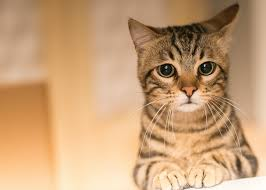
\includegraphics[width=0.4\textwidth]{gato.jpg}%
		\label{fig:gato}
	}
	\caption{Imagen de dos mascotas}
	\label{fig:mascotas}
\end{figure}